\apendice{Plan de Proyecto Software}

\section{Introducción}
Para el correcto desarrollo del proyecto se seguirá una planificacion temporal y se desarrollara una planificacion economica para ver el coste economico aproximado del producto desarrollado a lo largo del proyecto. Además, se dispondrá de un apartado donde consultar la viabilidad legal del desarrollo del proyecto.

\section{Planificación temporal}
% Inicio de la figura
\begin{figure}[h]
    \centering
    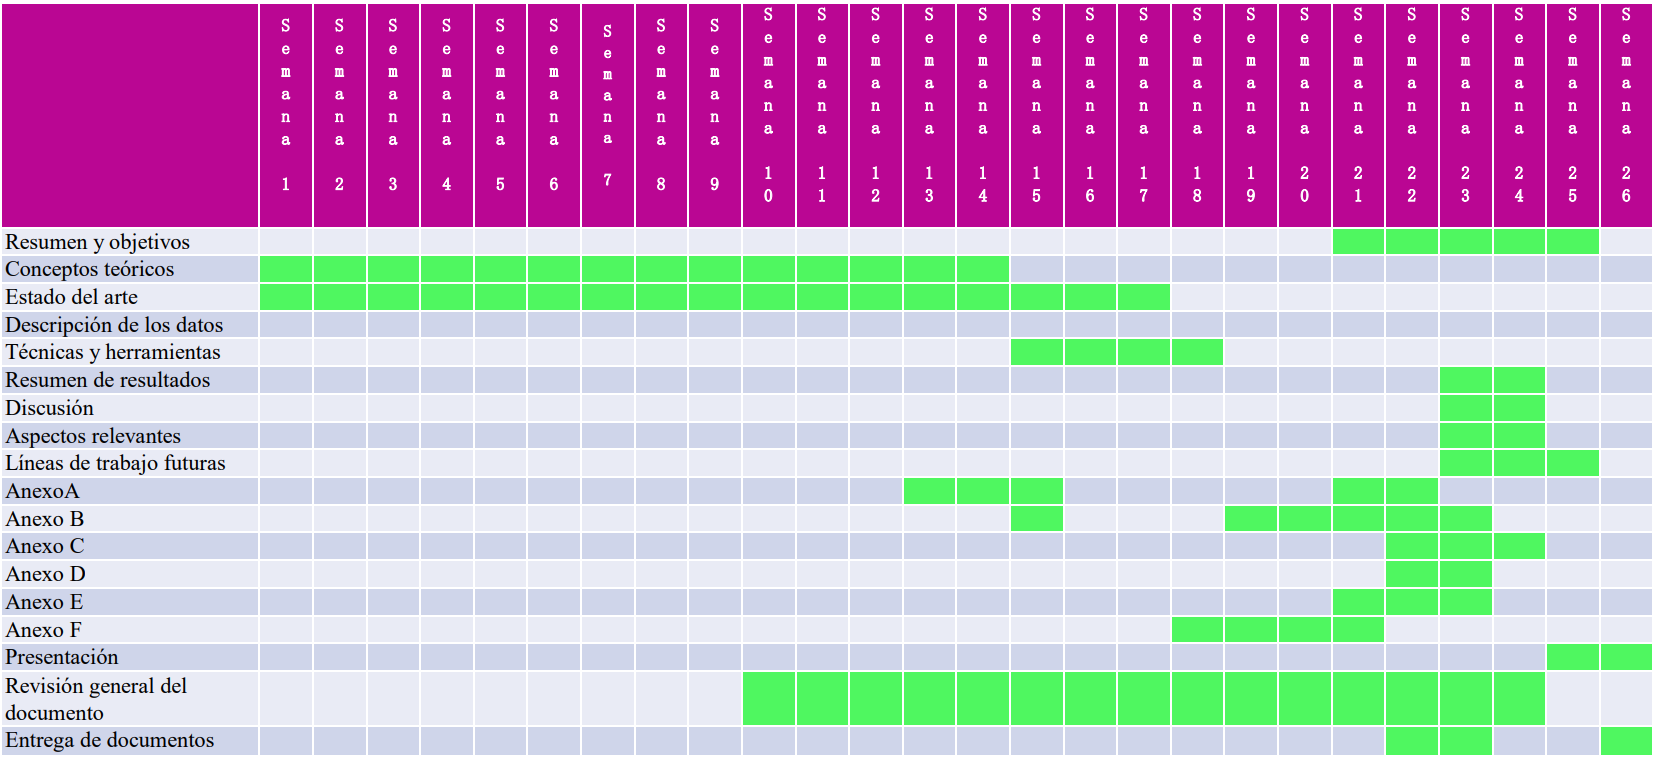
\includegraphics[width=1\textwidth]{img/PlanificacionTemporal.png}
    \caption{Planificación temporal seguida para la realización de este proyecto.}
    \label{fig:planTemporal} % Esta etiqueta es la que permite que se encuentr referenciada en el texto (es muy importante que siempre estén referenciadas en el texto)
\end{figure}
% Añadir una imagen con los hitos por semanas unas 14 semanas aprox aunque puede variar en funcion se vaya avanzando, en cuyo caso se volverá a modificar la tabla

En la planificación temporal se puede ver cada apartado de la memoria y los anexos desarrollados a lo largo de las semanas. 

\section{Planificación económica}
\textcolor{red}{falta incluir tiempo de desarrollo del ingeniero. SIEMPRE, porque sino estás diciendo que tu trabajo NO VALE NADA ...}

\textcolor{red}{también se incluyen los equipos  de desarrollo amortizados en 4 años, pero solo aplicando el tiempo de uso para el proyecto, es decir si son 4 o 6 meses esa parte proporcional de la amortización}

\textcolor{red}{quizás te pueden decir que los degloses mejor en tablas... pero no es importante.}

\textcolor{red}{y en los precios siempre hay que decir si con impuestos o sin impuestos. Tambíén te preguntarán por el proveedor...}

\textcolor{red}{en algunos casos en los costes se incluye el reciclado, aunque al no ser una producción industrial yo indicaria que se considera PROTOTIPO o PRE.serie pero nunca producción donde si hay que contemplarlo por legislación, creo.}

Para obtener una buena planificación económica se deberán identificar los gastos y los ingresos relacionados con el desarrollo del producto.

Como primeros gastos incluiremos el precio de los componentes y los gastos de producción, mientras que para obtener los ingresos se tendrá en cuenta el beneficio, gastos imprevistos e I+D del producto, para posibles mejoras en e futuro. La suma de gastos e ingresos nos devolverá el precio final del dispositivo.


% ----------------------------------------------------
% Tabla del desglose económico de las versiones realizadas.
\begin{table}[h!]
\centering
\begin{tabular}{ |m{4cm}|m{4cm}|m{2cm}|m{2cm}|  } 
\hline
\cellcolor[HTML]{B9E3F0}\textbf{} & \cellcolor[HTML]{B9E3F0}\textbf{Cálculos} & \cellcolor[HTML]{B9E3F0}\textbf{Versión 1}& \cellcolor[HTML]{B9E3F0}\textbf{Versión 2}\\

\hline
\cellcolor[HTML]{EFEFEF}\textbf{Gastos de los componentes}             & {Suma de los precios de cada componente del producto}   & 27€ & 32.5€\\
\hline
\cellcolor[HTML]{EFEFEF}\textbf{Gastos de producción}                & {10\% del precio de los componentes} & 2.7€ & 3.25€\\
\hline
\cellcolor[HTML]{EFEFEF}\textbf{Ingresos destinados a beneficio}                & {5\% del total de gastos} & 1.48€ & 1.79€\\
\hline
\cellcolor[HTML]{EFEFEF}\textbf{Gastos imprevistos e I+D} & {10\% del total de gastos} & 2.97€ & 3.58€\\
\hline
\cellcolor[HTML]{EFEFEF}\textbf{Precio Total} & {Suma de los gastos e ingresos} & \textbf{34.15€} & \textbf{41.10€}\\
\hline
\end{tabular}
\caption{Resumen de gastos y precio total del producto}
\end{table}

El prototipo de la versión 1, en la que se emplea el sensor SW520D, tiene un coste final aproximado\footnote{La planificación económica será variable en el tiempo y durante el desarrollo del producto, por lo que se trata de precios totales aproximados. Igual para el prototipo versión 2.} de unos 34.15€, precio que podría ser menor al crear nuestro propio microcontrolador o utilizar una alternativa similar a arduino, puesto que es el elemento que más aumenta el precio de la solución, siendo el precio del resto de los componentes aproximadamente unos 3€.

El prototipo de la versión 2, en la que se emplea el módulo MPU6050, tiene un coste final aproximado de unos 41.10€, precio que también podría disminuir al crear nuestro propio microcontrolador o utilizar una alternativa a arduino, ya que sin el microcontrolador Arduino el precio ronda los 8.5€.


\subsection{Desglose de los precios de los componentes del prototipo Versión 1}

Se han tenido en cuenta los precios más bajos encontrados de cada componente necesario.
\begin{itemize}
    \item Arduino UNO R3: 24€
    \item Resitencias (330 \textOmega, 2x220 \textOmega, 33 \textOmega, 1000 \textOmega): 0.05€
    \item Zumbador pasivo: 0.25€
    \item Motor de vibración: 1€
    \item Transistor: 0.05€
    \item SW520D: 0.5€
    \item Led azul: 0.02€
    \item Pulsador: 0.05€
    \item Otros elementos variados: 1€
    
\end{itemize}

\subsection{Desglose de los precios de los componentes del prototipo Versión 2}

Se han tenido en cuenta los precios más bajos encontrados de cada componente necesario.
\begin{itemize}
    \item Arduino UNO R3: 24€
    \item Resitencias (2x330 \textOmega, 2x220 \textOmega, 33 \textOmega, 1000 \textOmega): 0.06€
    \item Zumbador pasivo: 0.25€
    \item Motor de vibración: 1€
    \item Transistor NPN: 0.05€
    \item MPU-6050: 6€
    \item Led azul: 0.02€
    \item 2xPulsador: 0.10€
    \item Otros elementos variados: 1€
    
\end{itemize}




\section{Viabilidad legal}
\begin{comment}
Respecto a la viabilidad legal es respecto a que partes del desarrollo o comercialización  pueden pararse por problemas legales.

Datos almacenados de los usuarios.
\end{comment}

Se debe tener en cuenta en todo momento que el dispositivo sea completamente seguro y no afecte negativamente al usuario. Para ello, existen legislaciones específicas a cada fase del desarrollo y comercialización del producto que se deben cumplir para obtener un dispositivo seguro y regulado.

Se pueden diferenciar 3 fases, una primera fase de creación de la idea, diseño y desarrollo y realización de pruebas, una segunda fase de comercialización y la última fase de posventa, donde se incluyen las demandas y la gestión de los datos de los usuarios.

Durante la primera fase de creación de la idea, diseño y desarrollo del producto y realización de pruebas, todos los movimientos que se realicen se deberán ajustar a las siguientes legislaciones:
\begin{itemize}
    \item Ley 24/2015\cite{patentes}, Ley de Patentes, donde se regula todo lo relacionado con la protección de invenciones empleando patentes, desde el registro de las patentes, invenciones patentables, el derecho a la patente y los procedimientos para pedir una patente.
    % Referencia: 
    % https://www.boe.es/buscar/act.php?id=BOE-A-2015-8328
    
    \item Real Decreto Legislativo 1/1996\cite{PropIntelectual} relativo Ley de Propiedad Intelectual que regulariza la protección del derecho de autor y de derechos similares.
    % referencia:
    % https://boe.es/buscar/act.php?id=BOE-A-1996-8930
    
    \item Los productos sanitarios se rigen por la Agencia española de medicamentos y productos sanitarios (AEMPS)\cite{AEMPS}. En este proyecto nos interesan especialmente el Real Decreto 1591/2009\cite{prodSanitario1} que regula todo lo relativo a los productos sanitarios, desde su desarrollo a su venta, y el Real Decreto 437/2002\cite{prodSanitario2} establece las pautas para la concesión de licencias de fabricación y desarrollo de productos sanitarios.
    % Referencias:
    % https://www.aemps.gob.es/productos-sanitarios/legislacion-sobre-productos-sanitarios/
    % https://www.boe.es/buscar/doc.php?id=BOE-A-2009-17606
    % https://www.boe.es/buscar/doc.php?id=BOE-A-2002-10228
    
    \item Reglamento de la UE 2017/745\cite{ProdSanitariosEU} de Productos Sanitarios de la Union Europea este reglamento establece requisitos y regula la comercialización de productos sanitarios en la Unión Europea, con el fin de garantizar un dispositivo de calidad, eficaz y completamente seguro.
    % Referencia:
    % https://eur-lex.europa.eu/legal-content/ES/TXT/?uri=uriserv:OJ.L_.2017.117.01.0001.01.SPA&toc=OJ:L:2017:117:TOC
    
    \item Además, durante todo el desarrollo del producto se deberá cumplir con la normativa laboral española\cite{normaLaboral}, que incluye leyes y reglamentos como pueden ser el Estatuto de los Trabajadores, la Ley de Prevención de Riesgos Laborales o la Ley de Igualdad.
    % Referencia
    % https://www.boe.es/biblioteca_juridica/codigos/codigo.php?id=93&modo=2&nota=0&tab=2
    
\end{itemize}

Si se consigue crear el dispositivo en base a todas las leyes anteriores y se quisiera sacar a mercado se deberán cumplir también con los siguientes requisitos legales:
\begin{itemize}
    \item La Ley 34/2002\cite{comercioElectronico} de Servicios de la Sociedad de la Información y de Comercio Electrónico, en caso de que se realice una tienda web oficial de comercialización del dispositivo.
    % Referencia:
    % https://www.boe.es/buscar/act.php?id=BOE-A-2002-13758
    
    \item Además, se deberan tener en cuenta otras leyes\cite{comercio} como la Ley 7/1996\cite{comercioMinorista} de Ordenación del Comercio Minorista.
    % Referencia:
    % https://www.boe.es/buscar/act.php?id=BOE-A-1996-1072
    % https://www.boe.es/biblioteca_juridica/codigos/codigo.php?id=35&modo=2&nota=0&tab=2
\end{itemize}

Por último, si el dispositivo se ha puesto a la venta se debe pensar en los requisitos legales que se necesitarán cumplir a partir del momento de la primera venta. Alguno de estos requisitos serán:
\begin{itemize}
    \item Ley Orgánica 3/2018\cite{protDatos} de Protección de Datos Personales y garantía de los derechos digitales. Para poder proteger cualquier información que identifique a una persona, de forma confidencial. Además, el usuario debe estar correctamente informado del tratamiento de sus datos, ademas el acceso al tratamiento de sus datos debe ser claro y accesible.

    El usuario tendrá derecho al acceso de sus datos, derecho de rectificación y supresión de sus datos, derecho a la limitación del tratamiento de sus datos, derecho a la portabilidad de sus datos y el derecho a oponerse al tratamiento de sus datos. Por todo ello el tratamiento de sus datos debe ser tras la confirmación clara del consentimiento informado del tratamiento de sus datos.
    % Referencia:
    % https://www.boe.es/buscar/doc.php?id=BOE-A-2018-16673

    \item Reglamento UE 2016/679\cite{protDatosEU} relativo a Protección de las Personas Físicas en lo que respecta al tratamiento de datos personales y circulación de estos Datos. Donde se define que se debe garantizar la protección de los datos con los que se trabaja, además de notificar brechas de seguridad o exposición de datos al usuario.
    % Referencia:
    % https://eur-lex.europa.eu/ES/legal-content/summary/general-data-protection-regulation-gdpr.html
\end{itemize}


Además el dispositivo deberá contar con un certificado CE\cite{certificadoEuropeo}, que garantizará que el dispositivo cumple con los requisitos de seguridad, protección y sanidad europeos. Una vez se obtenga el certificado el dispositivo podrá ser comercializado legalmente en la Unión Europea.
% Referencia:
% https://europa.eu/youreurope/business/product-requirements/labels-markings/ce-marking/index_es.htm